\documentclass{jsarticle}

    \usepackage{amsmath,amssymb}
    \usepackage{bm}
    \usepackage{braket}
    \usepackage[dvipdfmx]{graphicx}
    \usepackage{here}
    \makeatletter
    \c@MaxMatrixCols=12
    \makeatother
    
    \begin{document}
    \part{BdGモデルハミルトニアンについて}
        \section{定義}
            BdGモデルハミルトニアン$\mathcal{H}$は以下のように表される。
    
            \begin{align}
                \mathcal{H}=\int \vec{\Psi}^\dagger \tilde{H}\vec{\Psi}dr
                \label{hamil0}
            \end{align}
    
            \begin{align}
                \int dr=\int dxdy
            \end{align}
    
            \begin{align}
                \vec{\Psi}=
                \begin{bmatrix}
                    \Psi_\uparrow \\
                    \Psi_\downarrow \\
                    \Psi_\uparrow^\dagger \\
                    \Psi_\downarrow^\dagger
                \end{bmatrix}
            \end{align}
    
            \begin{align}
                \tilde{H}=
                \begin{bmatrix}
                    \hat{h}(r) & \hat{\Delta}(r) \\
                    -\hat{\Delta}^\ast(r) & -\hat{h}^\ast(r)
                \end{bmatrix}
            \end{align}
    
            \begin{align}
                \hat{h}=\left[-\frac{\hbar^2}{2m}\nabla^2-\mu_F \right]\hat{\sigma}_0 \\
                \left( \hat{\sigma}_0:単位行列 \right)
            \end{align}
    
            \begin{align}
                \hat{\Delta}(r)=
                \begin{cases}
                    \Delta_0 \left( i \hat{\sigma}_2 \right) & \mbox{s-wave} \\
                    \Delta_0\frac{i\partial x}{k_F}\hat{\sigma}_1 & \mbox{ $p_x$-wave} \\
                    \Delta_0\frac{1}{k_f} \left( \hat{\sigma}_1+i\hat{\sigma}_2 \right) & \mbox{$p_x+ip_y$}
                \end{cases}
                \label{Delta}
            \end{align}
    
            \begin{align}
                \vec{\Psi}=\frac{1}{\sqrt{L_y}}\sum_{k_y} \vec{\Psi}_{k_y}(x) e^{ik_yy}
                \label{fourier}
            \end{align}
    
            \begin{figure}[H]
                \centering
                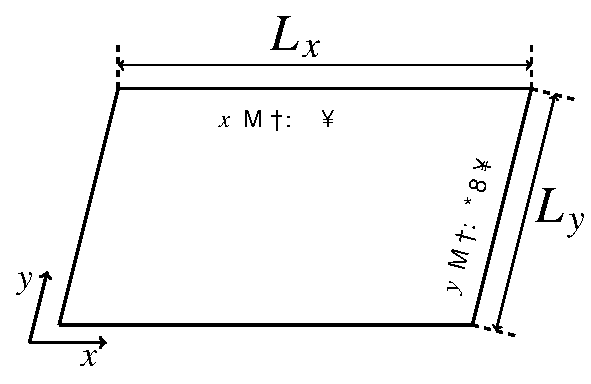
\includegraphics[scale=1]{figure1}
                \caption{考える系}
                \label{system}
            \end{figure}
    
        \section{問題}
            \subsection{ハミルトニアン $\mathcal{H}$ をフーリエ変換せよ}
            式\eqref{hamil0}に式\eqref{fourier}を代入して計算していく。

            ここで
    
            \begin{align}
                \hat{\sigma}_0=
                \begin{bmatrix}
                    1 & 0 \\
                    0 & 1
                \end{bmatrix},
                \hat{\sigma}_1=
                \begin{bmatrix}
                    0 & 1 \\
                    1 & 0
                \end{bmatrix},
                \hat{\sigma}_2=
                \begin{bmatrix}
                    0 & -i \\
                    i & 0
                \end{bmatrix} ,
                \hat{\sigma}_3=
                \begin{bmatrix}
                    1 & 0 \\
                    0 & -1
                \end{bmatrix}
            \end{align}

            とする。
            
        \subsubsection{s-waveのとき}
    	このとき、$\hat{\Delta}(r)=\Delta_0 \left( i \hat{\sigma}_2 \right)$となるため、
    	
    		
            \begin{align}
                \mathcal{H}=\int \int \left( \frac{1}{\sqrt{L_y}}\sum_{k_y} \vec{\Psi}^\dagger _{k_y}(x) e^{-ik_yy} \right) \tilde{H} \left( \frac{1}{\sqrt{L_y}}\sum_{k_y'} \vec{\Psi}_{k_y'}(x) e^{ik_y'y} \right) dxdy
                \label{hamil}
            \end{align}
    
            よって、ハミルトニアン$\mathcal{H}$は、
    
            \begin{align}
                \mathcal{H}=
                \begin{bmatrix}
                    -\frac{\hbar^2}{2m}\nabla^2-\mu_F & 0 & 0 & \Delta_0 \\
                    0 & -\frac{\hbar^2}{2m}\nabla^2-\mu_F & -\Delta_0 & 0 \\
                    0 & -\Delta_0^\ast & \frac{\hbar^2}{2m}\nabla^2+\mu_F & 0 \\
                    \Delta_0^\ast & 0 & 0 & \frac{\hbar^2}{2m}\nabla^2+\mu_F
                \end{bmatrix}
            \end{align}
    
            これを、式\eqref{hamil}に代入して計算していく。 \\
            このとき、
    
            \begin{align}
                \vec{\Psi}_{k_y}^\dagger(x) e^{-ik_yy} \tilde{H}  \vec{\Psi}_{k_y'}(x) e^{ik_y'y} =
                e^{-ik_yy} \left[ \Psi_\uparrow^\dagger \left( -\frac{\hbar^2}{2m}\nabla^2-\mu_F \right) +\Psi_\downarrow^\dagger \Delta_0^\ast \right] \Psi_\uparrow e^{ik'_yy} \nonumber\\
                +e^{-ik_yy} \left[ \Psi_\downarrow^\dagger \left( -\frac{\hbar^2}{2m}\nabla^2-\mu_F \right) -\Psi_\uparrow^\dagger \Delta_0^\ast \right] \Psi_\downarrow e^{ik'_yy} \nonumber\\
                + e^{-ik_yy} \left[ -\Psi_\downarrow\Delta_0 +\Psi_\uparrow \left( \frac{\hbar^2}{2m}\nabla^2+\mu_F \right) \right] \Psi_\uparrow^\dagger e^{ik'_yy} \nonumber\\
                +e^{-ik_yy} \left[ \Psi_\uparrow\Delta_0 +\Psi_\downarrow \left( \frac{\hbar^2}{2m}\nabla^2+\mu_F \right) \right] \Psi_\downarrow^\dagger e^{ik'_yy}
            \end{align}
    
            また、
    
            \begin{align}
            \int \left( \sum_{k_y}\sum_{k'_y}\Psi^\dagger(k) e^{-ik_yy}\Psi(k')e^{ik_y'y} \right) dy \nonumber \\
            =L_y\sum_{k_y}\sum_{k'_y}\Psi^\dagger(k) \Psi(k')\delta \left( k-k' \right) \nonumber \\
            =L_y\sum_{k_y}\Psi^\dagger(k)\Psi(k)
            \end{align}
    
            \begin{align}
                \nabla^2 \left[ \Psi_\uparrow e^{ik'_yy} \right]=
                \frac{\hbar^2}{2m}
                \left( -k_y^2\Psi e^{ik'_yy} + e^{ik'_yy}\frac{\partial^2}{\partial x^2}\Psi \right)
            \end{align}
    
    
            から、式\eqref{hamil}は、
    
            \begin{align}
                \mathcal{H}=\int dx \sum_{k_y}
                \left[ \Psi_\uparrow^\dagger \left( \frac{\hbar^2k_y^2}{2m}-\mu_F \right)\Psi_\uparrow
                +\Psi_\uparrow^\dagger \left(- \frac{\hbar^2}{2m}\frac{\partial^2}{\partial x^2}\right)\Psi_\uparrow
                +\Psi_\downarrow^\dagger \Delta_0^\ast \Psi_\uparrow \right. \nonumber \\ \left.+
                \Psi_\downarrow^\dagger \left( \frac{\hbar^2k_y^2}{2m}-\mu_F \right)\Psi_\downarrow
                +\Psi_\downarrow^\dagger \left(- \frac{\hbar^2}{2m}\frac{\partial^2}{\partial x^2} \right) \Psi_\downarrow
                -\Psi_\uparrow^\dagger \Delta_0^\ast \Psi_\downarrow \cdots
                \right]
                \label{hamil1}
            \end{align}
            
            \subsubsection{$P_x$-waveのとき}
             今度は、$\hat{\Delta}(r)=\Delta_0\frac{1}{k_f} \left( \partial x+i\partial y \right)\hat{\sigma}_1$のときを考える。

            ハミルトニアンの式は、
            
            \begin{align}
                \mathcal{H}=
                \begin{bmatrix}
                    -\frac{\hbar^2}{2m}\nabla^2-\mu_F & 0 & 0 & \Delta_0\frac{i\partial x}{k_F} \\
                    0 & -\frac{\hbar^2}{2m}\nabla^2-\mu_F & \Delta_0\frac{i\partial x}{k_F} & 0 \\
                    0 & \Delta_0^\ast\frac{i\partial x}{k_F} & \frac{\hbar^2}{2m}\nabla^2+\mu_F & 0 \\
                     \Delta_0^\ast\frac{i\partial x}{k_F} & 0 & 0 & \frac{\hbar^2}{2m}\nabla^2+\mu_F
                \end{bmatrix}
            \end{align}
    
            これを、式\eqref{hamil}に代入して計算していく。 \\
    
            以下
            \begin{align}
                \eta=\Delta_0\frac{i\partial x}{k_F} \\
                \eta^{'}=\Delta_0^\ast\frac{i\partial x}{k_F}
            \end{align}
            とする。

            最初のものと同様に計算し、

            \begin{align}
                \mathcal{H}=\int dx \sum_{k_y}
                \left[ \Psi_\uparrow^\dagger \left( \frac{\hbar^2k_y^2}{2m}-\mu_F \right)\Psi_\uparrow
                +\Psi_\uparrow^\dagger \left(- \frac{\hbar^2}{2m}\frac{\partial^2}{\partial x^2}\right)\Psi_\uparrow
                +\Psi_\downarrow^\dagger \eta \Psi_\uparrow \right. \nonumber \\ \left.+
                \Psi_\downarrow^\dagger \left( \frac{\hbar^2k_y^2}{2m}-\mu_F \right)\Psi_\downarrow
                +\Psi_\downarrow^\dagger \left(- \frac{\hbar^2}{2m}\frac{\partial^2}{\partial x^2} \right) \Psi_\downarrow
                -\Psi_\uparrow^\dagger \eta \Psi_\downarrow \cdots
                \right]
                \label{hamil2}
            \end{align}

            \subsubsection{$P_x+iP_y$のとき}
             今度は、$\hat{\Delta}(r)=\Delta_0\frac{1}{k_f} \left( \partial x+i\partial y \right)\hat{\sigma}_1$のときを考える。

            ハミルトニアンの式は、

            \begin{align}
                \mathcal{H}=
                \begin{bmatrix}
                    -\frac{\hbar^2}{2m}\nabla^2-\mu_F & 0 & 0 & \Delta_0\frac{1}{k_f} \left( \partial x+i\partial y \right) \\
                    0 & -\frac{\hbar^2}{2m}\nabla^2-\mu_F & \Delta_0\frac{1}{k_f} \left( \partial x+i\partial y \right) & 0 \\
                    0 & -\Delta_0^\ast\frac{1}{k_f} \left( \partial x-i\partial y \right) & \frac{\hbar^2}{2m}\nabla^2+\mu_F & 0 \\
                     -\Delta_0^\ast\frac{1}{k_f} \left( \partial x-i\partial y \right) & 0 & 0 & \frac{\hbar^2}{2m}\nabla^2+\mu_F
                \end{bmatrix}
            \end{align}

            以下
		    \begin{align}
			    \xi=\Delta_0\frac{1}{k_f} \\
			    \xi^{'}=\Delta_0^\ast\frac{1}{k_f}
		    \end{align}
            とする
            
            最初のものと同様に計算し、

            \begin{align}
                \mathcal{H}=\int dx \sum_{k_y}
                \left[ \Psi_\uparrow^\dagger \left( \frac{\hbar^2k_y^2}{2m}-\mu_F \right)\Psi_\uparrow
                +\Psi_\uparrow^\dagger \left(- \frac{\hbar^2}{2m}\frac{\partial^2}{\partial x^2}\right)\Psi_\uparrow
                +\Psi_\downarrow^\dagger \xi\left( \partial x-k_y \right) \Psi_\uparrow \right. \nonumber \\ \left.+
                \Psi_\downarrow^\dagger \left( \frac{\hbar^2k_y^2}{2m}-\mu_F \right)\Psi_\downarrow
                +\Psi_\downarrow^\dagger \left(- \frac{\hbar^2}{2m}\frac{\partial^2}{\partial x^2} \right) \Psi_\downarrow
                +\Psi_\uparrow^\dagger \xi \left( \partial x-k_y \right) \Psi_\downarrow \cdots
                \right]
                \label{hamil3}
            \end{align}


            \subsection{差分近似をしよう}
            刻み幅を1として、差分近似をする。微小変化$h$周りにマクローリン展開を行うと、
    
            \begin{align}
                \Psi\left(x+h\right)=\Psi\left(x\right)+h\frac{\partial}{\partial x}\Psi\left(x\right)+\frac{h^2}{2!}\frac{\partial^2}{\partial x^2}\Psi\left(x\right)
                \label{macro+}
            \end{align}
    
            \begin{align}
                \Psi\left(x-h\right)=\Psi\left(x\right)-h\frac{\partial}{\partial x}\Psi\left(x\right)+\frac{h^2}{2!}\frac{\partial^2}{\partial x^2}\Psi\left(x\right)
                \label{macro-}
            \end{align}
    
            よって、差分近似は式\eqref{macro+},式\eqref{macro-}の方程式で求めることができ、刻み幅$h=1$とすると、
    
            \begin{align}
                \frac{\partial}{\partial x}\Psi\left(x\right)=
                \frac{\Psi\left(x+1\right)-\Psi\left(x-1\right)}{2}
            \end{align}
    
            \begin{align}
                \frac{\partial^2}{\partial x^2}\Psi\left(x\right)=
                \Psi\left(x+1\right)-2\Psi\left(x\right)+\Psi\left(x-1\right)
                \label{macro2}
            \end{align}
    
            \subsection{xを離散化せよ}
            式\eqref{macro2}を式\eqref{hamil1}、\eqref{hamil2}、\eqref{hamil3}に代入して、行列で表す。このとき、離散化した波動関数を以下の式に定義する。
            
            \begin{align}
                \vec{\Psi}=
                \begin{bmatrix}
                    \Psi_{1\uparrow} \\
                    \Psi_{1\downarrow} \\
                    \Psi_{1\uparrow}^\dagger \\
                    \Psi_{1\downarrow}^\dagger \\
                    \Psi_{2\uparrow} \\
                    \cdot \\
                    \cdot
                \end{bmatrix},
                \Psi_{n\pm 1\uparrow}=\Psi_{n\uparrow}\left(x\pm 1\right)
            \end{align}
    
            \subsubsection{s-waveのとき}
            代入した式は、
    
            \begin{align}
                \mathcal{H}= \sum_{i=1}^N \sum_{k_y}
                \left[ \Psi^\dagger_{i\uparrow} \left( \frac{\hbar^2k_y^2}{2m}-\mu_F \right)\Psi_{i\uparrow}
                +\Psi^\dagger_{i\uparrow} \left( \Psi_{i+1\uparrow}\left(x\right)-2\Psi_{i\uparrow}\left(x\right)+\Psi_{i-1\uparrow}\left(x\right)
                \right)+\Psi^\dagger_{i\downarrow} \Delta_0^\ast \Psi_{i\uparrow} \cdots
                \right]
                \label{hamil'}
            \end{align}
    
            $N=3$と置くとき、ハミルトニアンを2次形式で表すと、
            
            \begin{align}
                \mathcal{H}=
                \begin{bmatrix}
                    \Psi_{1\uparrow}^\dagger \\
                    \Psi_{1\downarrow}^\dagger \\
                    \Psi_{1\uparrow} \\
                    \Psi_{1\downarrow} \\
                    \Psi_{2\uparrow}^\dagger \\
                    \Psi_{2\downarrow}^\dagger \\
                    \Psi_{2\uparrow} \\
                    \Psi_{2\downarrow} \\
                    \Psi_{3\uparrow}^\dagger \\
                    \Psi_{3\downarrow}^\dagger \\
                    \Psi_{3\uparrow} \\
                    \Psi_{3\downarrow}
                \end{bmatrix}
                ^T
                \begin{bmatrix}
                    \varepsilon_{k_y} & 0 & 0 & \Delta_0 & -\varLambda & 0 & 0 & 0 & 0 & 0 & 0 & 0 \\
                    0 & \varepsilon_{k_y} & -\Delta_0 & 0 & 0 & -\varLambda & 0 & 0 & 0 & 0 & 0 & 0 \\
                    0 & -\Delta_0^\ast & -\varepsilon_{k_y} & 0 & 0 & 0 & \varLambda & 0 & 0 & 0 & 0 & 0 \\
                    \Delta_0^\ast & 0 & 0 & -\varepsilon_{k_y} & 0 & 0 & 0 & \varLambda & 0 & 0 & 0 & 0 \\
                    -\varLambda & 0 & 0 & 0 & \varepsilon_{k_y} & 0 & 0 & \Delta_0 & -\varLambda & 0 & 0 & 0 \\
                    0 & -\varLambda & 0 & 0 & 0 & \varepsilon_{k_y} & -\Delta_0 & 0 & 0 & -\varLambda & 0 & 0 \\
                    0 & 0 & \varLambda & 0 & 0 & -\Delta_0^\ast & -\varepsilon_{k_y} & 0 & 0 & 0 & \varLambda & 0 \\
                    0 & 0 & 0 & \varLambda & \Delta_0^\ast & 0 & 0 & -\varepsilon_{k_y} & 0 & 0 & 0 & \varLambda \\
                    0 & 0 & 0 & 0 & -\varLambda & 0 & 0 & 0 & \varepsilon_{k_y} & 0 & 0 & \Delta_0 \\
                    0 & 0 & 0 & 0 & 0 & -\varLambda & 0 & 0 & 0 & \varepsilon_{k_y} & -\Delta_0 & 0 \\
                    0 & 0 & 0 & 0 & 0 & 0 & \varLambda & 0 & 0 & -\Delta_0^\ast & -\varepsilon_{k_y} & 0 \\
                    0 & 0 & 0 & 0 & 0 & 0 & 0 & \varLambda & -\Delta_0^\ast & 0 & 0 & -\varepsilon_{k_y}
                \end{bmatrix}
                \begin{bmatrix}
                    \Psi_{1\uparrow} \\
                    \Psi_{1\downarrow} \\
                    \Psi_{1\uparrow}^\dagger \\
                    \Psi_{1\downarrow}^\dagger \\
                    \Psi_{2\uparrow} \\
                    \Psi_{2\downarrow} \\
                    \Psi_{2\uparrow}^\dagger \\
                    \Psi_{2\downarrow}^\dagger \\
                    \Psi_{3\uparrow} \\
                    \Psi_{3\downarrow} \\
                    \Psi_{3\uparrow}^\dagger \\
                    \Psi_{3\downarrow}^\dagger \\
                \end{bmatrix}
            \end{align}
    
            ここで
    
            \begin{align}
                \varepsilon_{k_y}=\frac{\hbar^2}{2m}(k_y^2+2)-\mu_F
            \end{align}
    
            \begin{align}
                \varLambda=\frac{\hbar^2}{2m}
            \end{align}
    
            とおく

            \subsubsection{$P_x$-waveのとき}

            代入した式は、

		    \begin{align}
			    \mathcal{H}= \sum_{i=1}^N \sum_{k_y}
			    \left[ \Psi^\dagger_{i\uparrow} \left( \frac{\hbar^2k_y^2}{2m}-\mu_F \right)\Psi_{i\uparrow}
			    +\Psi^\dagger_{i\uparrow} \left( \Psi_{i+1\uparrow}\left(x\right)-2\Psi_{i\uparrow}\left(x\right)+\Psi_{i-1\uparrow}\left(x\right)
			    \right)+\Psi^\dagger_{i\downarrow} \Delta_0^\ast \Psi_{i\uparrow} \cdots
			    \right]
		    \end{align}

		    このとき、$\eta$ のなかの微分を考慮する。
		    $N=3$と置くとき、ハミルトニアンを2次形式で表すと、

		    \begin{align}
			    \mathcal{H}=
			    \begin{bmatrix}
				    \Psi_{1\uparrow}^\dagger \\
				    \Psi_{1\downarrow}^\dagger \\
				    \Psi_{1\uparrow} \\
			    	\Psi_{1\downarrow} \\
				    \Psi_{2\uparrow}^\dagger \\
				    \Psi_{2\downarrow}^\dagger \\
			    	\Psi_{2\uparrow} \\
			    	\Psi_{2\downarrow} \\
			    	\Psi_{3\uparrow}^\dagger \\
			    	\Psi_{3\downarrow}^\dagger \\
			    	\Psi_{3\uparrow} \\
			    	\Psi_{3\downarrow}
			    \end{bmatrix}
			    ^T
			    \begin{bmatrix}
			    	\varepsilon_{k_y} & 0 & 0 & 0 & -\varLambda & 0 & 0 & \zeta & 0 & 0 & 0 & 0 \\
			    	0 & \varepsilon_{k_y} & 0 & 0 & 0 & -\varLambda & \zeta & 0 & 0 & 0 & 0 & 0 \\
			    	0 & 0 & -\varepsilon_{k_y} & 0 & 0 & \zeta^{'} & \varLambda & 0 & 0 & 0 & 0 & 0 \\
			    	0 & 0 & 0 & -\varepsilon_{k_y} & \zeta^{'} & 0 & 0 & \varLambda & 0 & 0 & 0 & 0 \\
			    	-\varLambda & 0 & 0 & -\zeta & \varepsilon_{k_y} & 0 & 0 & 0 & -\varLambda & 0 & 0 & \zeta \\
			    	0 & -\varLambda & -\zeta & 0 & 0 & \varepsilon_{k_y} & 0 & 0 & 0 & -\varLambda & \zeta & 0 \\
			    	0 & -\zeta^{'} & \varLambda & 0 & 0 & 0 & -\varepsilon_{k_y} & 0 & 0 & \zeta^{'} & \varLambda & 0 \\
			    	-\zeta^{'} & 0 & 0 & \varLambda & 0 & 0 & 0 & -\varepsilon_{k_y} & \zeta^{'} & 0 & 0 & \varLambda \\
			    	0 & 0 & 0 & 0 & -\varLambda & 0 & 0 & -\zeta & \varepsilon_{k_y} & 0 & 0 & 0 \\
			    	0 & 0 & 0 & 0 & 0 & -\varLambda & -\zeta & 0 & 0 & \varepsilon_{k_y} & 0 & 0 \\
			    	0 & 0 & 0 & 0 & 0 & -\zeta^{'} & \varLambda & 0 & 0 & 0 & -\varepsilon_{k_y} & 0 \\
			    	0 & 0 & 0 & 0 & -\zeta^{'} & 0 & 0 & \varLambda & 0 & 0 & 0 & -\varepsilon_{k_y}
			    \end{bmatrix}
			    \begin{bmatrix}
			    	\Psi_{1\uparrow} \\
			    	\Psi_{1\downarrow} \\
			    	\Psi_{1\uparrow}^\dagger \\
			    	\Psi_{1\downarrow}^\dagger \\
			    	\Psi_{2\uparrow} \\
			    	\Psi_{2\downarrow} \\
			    	\Psi_{2\uparrow}^\dagger \\
			    	\Psi_{2\downarrow}^\dagger \\
			    	\Psi_{3\uparrow} \\
			    	\Psi_{3\downarrow} \\
			    	\Psi_{3\uparrow}^\dagger \\
			    	\Psi_{3\downarrow}^\dagger \\
			    \end{bmatrix}
		    \end{align}

		    ここで

		    \begin{align}
		    	\varepsilon_{k_y}=\frac{\hbar^2}{2m}(k_y^2+2)-\mu_F \\
		    	\varLambda=\frac{\hbar^2}{2m}\\
		    	\zeta=\dfrac{\Delta_0}{2k_{F}}i\\
		    	\zeta^{'}=\dfrac{\Delta_0^{*}}{2k_{F}}i\\
		    	\mu=\dfrac{\hbar^{2}k_F^{2}}{2m}
		    \end{align}

		    とおく

            \subsubsection{$P_x+iP_y$のとき}

            微分を考慮する。
		    $N=3$と置くとき、ハミルトニアンを2次形式で表すと、

		    \begin{align}
		    	\mathcal{H}=
		    	\begin{bmatrix}
		    		\Psi_{1\uparrow}^\dagger \\
		    		\Psi_{1\downarrow}^\dagger \\
		    		\Psi_{1\uparrow} \\
		    		\Psi_{1\downarrow} \\
		    		\Psi_{2\uparrow}^\dagger \\
		    		\Psi_{2\downarrow}^\dagger \\
		    		\Psi_{2\uparrow} \\
		    		\Psi_{2\downarrow} \\
		    		\Psi_{3\uparrow}^\dagger \\
		    		\Psi_{3\downarrow}^\dagger \\
		    		\Psi_{3\uparrow} \\
		    		\Psi_{3\downarrow}
		    	\end{bmatrix}
		    	^T
		    	\begin{bmatrix}
		    		\varepsilon_{k_y} & 0 & 0 & -k_y\xi & -\varLambda & 0 & 0 & \zeta & 0 & 0 & 0 & 0 \\
		    		0 & \varepsilon_{k_y} & -k_y\xi & 0 & 0 & -\varLambda & \zeta & 0 & 0 & 0 & 0 & 0 \\
		    		0 & -k_y\xi^{'} & -\varepsilon_{k_y} & 0 & 0 & -\zeta^{'} & \varLambda & 0 & 0 & 0 & 0 & 0 \\
		    		-k_y\xi^{'} & 0 & 0 & -\varepsilon_{k_y} & -\zeta^{'} & 0 & 0 & \varLambda & 0 & 0 & 0 & 0 \\
		    		-\varLambda & 0 & 0 & -\zeta & \varepsilon_{k_y} & 0 & 0 & -k_y\xi & -\varLambda & 0 & 0 & \zeta \\
		    		0 & -\varLambda & -\zeta & 0 & 0 & \varepsilon_{k_y} & -k_y\xi & 0 & 0 & -\varLambda & \zeta & 0 \\
		    		0 & \zeta^{'} & \varLambda & 0 & 0 & -k_y\xi^{'} & -\varepsilon_{k_y} & 0 & 0 & -\zeta^{'} & \varLambda & 0 \\
		    		\zeta^{'} & 0 & 0 & \varLambda & -k_y\xi^{'} & 0 & 0 & -\varepsilon_{k_y} & -\zeta^{'} & 0 & 0 & \varLambda \\
		    		0 & 0 & 0 & 0 & -\varLambda & 0 & 0 & -\zeta & \varepsilon_{k_y} & 0 & 0 & -k_y\xi \\
		    		0 & 0 & 0 & 0 & 0 & -\varLambda & -\zeta & 0 & 0 & \varepsilon_{k_y} & -k_y\xi & 0 \\
		    		0 & 0 & 0 & 0 & 0 & \zeta^{'} & \varLambda & 0 & 0 & -k_y\xi^{'} & -\varepsilon_{k_y} & 0 \\
		    		0 & 0 & 0 & 0 & \zeta^{'} & 0 & 0 & \varLambda & -k_y\xi^{'} & 0 & 0 & -\varepsilon_{k_y}
		    	\end{bmatrix}
		    	\begin{bmatrix}
		    		\Psi_{1\uparrow} \\
		    		\Psi_{1\downarrow} \\
		    		\Psi_{1\uparrow}^\dagger \\
		    		\Psi_{1\downarrow}^\dagger \\
		    		\Psi_{2\uparrow} \\
		    		\Psi_{2\downarrow} \\
		    		\Psi_{2\uparrow}^\dagger \\
		    		\Psi_{2\downarrow}^\dagger \\
		    		\Psi_{3\uparrow} \\
		    		\Psi_{3\downarrow} \\
		    		\Psi_{3\uparrow}^\dagger \\
		    		\Psi_{3\downarrow}^\dagger \\
		    	\end{bmatrix}
		    \end{align}

	    	ここで  

	    	\begin{align}
	    		\varepsilon_{k_y}=\frac{\hbar^2}{2m}(k_y^2+2)-\mu_F \\
		    	\varLambda=\frac{\hbar^2}{2m}\\
			    \zeta=\dfrac{\Delta_0}{2k_{F}}\\
		    	\zeta^{'}=\dfrac{\Delta_0^{*}}{2k_{F}}\\
		    	\mu=\dfrac{\hbar^{2}k_F^{2}}{2m}\\
		    	\xi=\Delta_0\frac{1}{k_f} \\
		    	\xi^{'}=\Delta_0^\ast\frac{1}{k_f}
		    \end{align}

		とおく

    
            \section{結果}
            $\mathcal{H}$を数値計算で対角化し、次に、グリーン関数を用いて状態密度を求めた。

            グリーン関数は、以下の通りである。
    
            \begin{align}
                G=(E+i\delta-H)^(-1)
                \label{Green}
            \end{align}

            式\eqref{Green}を用いると、表面の状態密度は
    
            \begin{align}
                \rho=-\frac{1}{\pi}Im(G_{11}+G_{22})
            \end{align}
    
            で表される。

            \subsubsection{s-waveのとき}
            $N=100$、$k_y$を横軸、固有値を縦軸として分散関係をプロットした。結果は以下のとおりである。
    
            \begin{figure}[H]
                \centering
                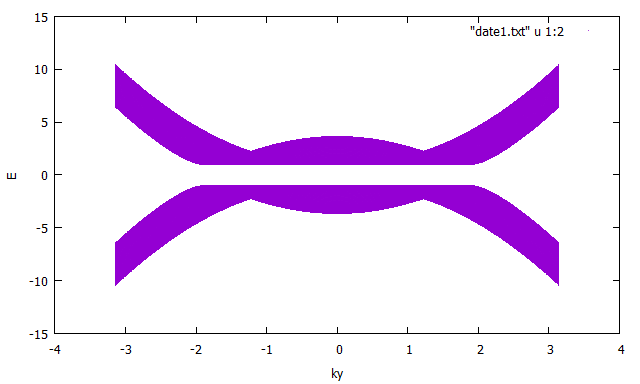
\includegraphics[scale=0.5]{BdG_bry.png}
                \caption{分散関係1}
                \label{Dispersion1}
            \end{figure}
    
            $E$を$-3$から$3$の範囲で動かし、$\rho$をプロットした。このとき$\delta=10^{-3}$とした。
            表面の時とバルクの時の結果を以下に示す。
    
            \begin{figure}[H]
                \centering
                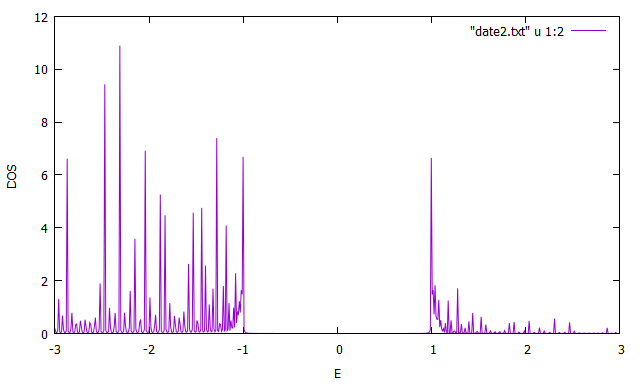
\includegraphics[scale=0.5]{LDOS_bry.png}
                \caption{状態密度1(表面)}
                \label{LDOS1}
            \end{figure}

            \begin{figure}[H]
                \centering
                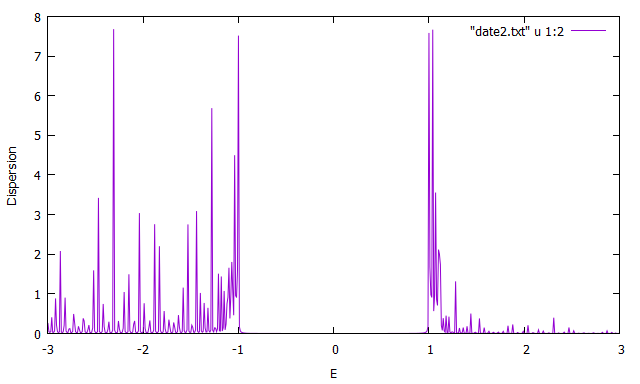
\includegraphics[scale=0.5]{LDOSb_bry.png}
                \caption{状態密度1(バルク)}
                \label{LDOS1b}
            \end{figure}
    
            図\eqref{LDOS1}から、表面はエネルギーが$-1$から$1$の範囲では状態がないことが分かる。また、表面とバルクで大きな違いはないこともわかる。ゆえに、エッジ状態はないと考えられる。
    
            \subsubsection{$P_x$-waveのとき}
            $N=100$、$k_y$を横軸、固有値を縦軸として分散関係をプロットした。結果は以下のとおりである。
    
            \begin{figure}[H]
                \centering
                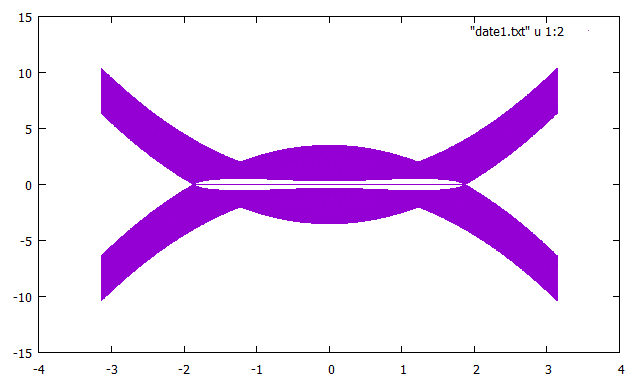
\includegraphics[scale=0.5]{BdG2_bry.png}
                \caption{分散関係2}
                \label{Dispersion2}
            \end{figure}
    
            次に、グリーン関数を用いて状態密度を求める。
            
            $E$を$-3$から$3$の範囲で動かし、$\rho$をプロットした。このとき$\delta=10^{-3}$とした。
            表面の時とバルクの時の結果を以下に示す。
    
            \begin{figure}[H]
                \centering
                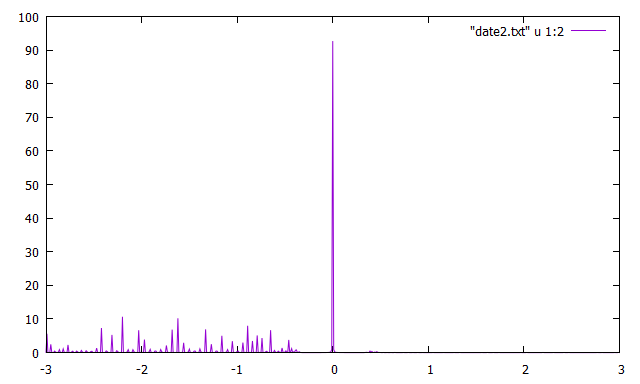
\includegraphics[scale=0.5]{LDOS2.png}
                \caption{状態密度2(表面)}
                \label{LDOS2}
            \end{figure}

            \begin{figure}[H]
                \centering
                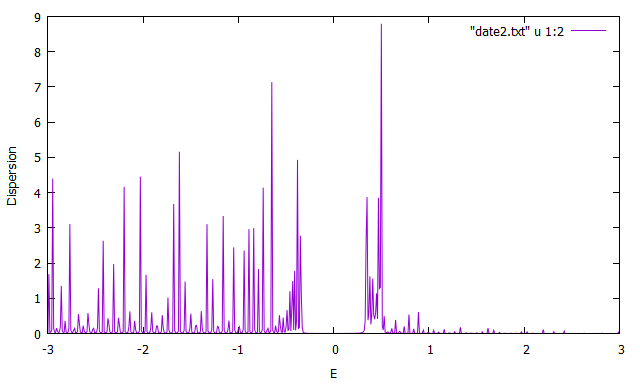
\includegraphics[scale=0.5]{LDOS2b.png}
                \caption{状態密度2(バルク)}
                \label{LDOS2b}
            \end{figure}

            図\eqref{LDOS2}から、表面ではE=0のときにピークが出ているのが分かる。それに対し図\eqref{LDOS2b}から、エネルギーが$-1$から$1$の範囲では状態がないことが分かる。これは、表面にエッジ状態があり、そこに電子が入ったためと考えられる。エッジ状態があるのは、図\eqref{Dispersion2}からも確認できる。
    
            \subsubsection{$P_x+iP_y$のとき}
            $N=100$、$k_y$を横軸、固有値を縦軸として分散関係をプロットした。結果は以下のとおりである。
    
            \begin{figure}[H]
                \centering
                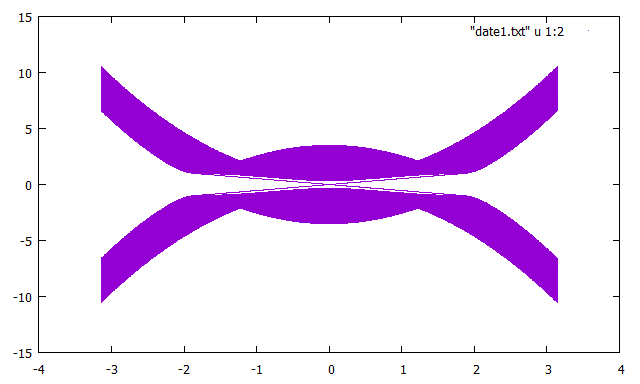
\includegraphics[scale=0.5]{BdG3_bry.png}
                \caption{分散関係3}
                \label{Dispersion3}
            \end{figure}
    
            次に、グリーン関数を用いて状態密度を求める。
           
            $E$を$-3$から$3$の範囲で動かし、$\rho$をプロットした。このとき$\delta=10^{-3}$とした。
            表面の時とバルクの時の結果を以下に示す。
    
            \begin{figure}[H]
                \centering
                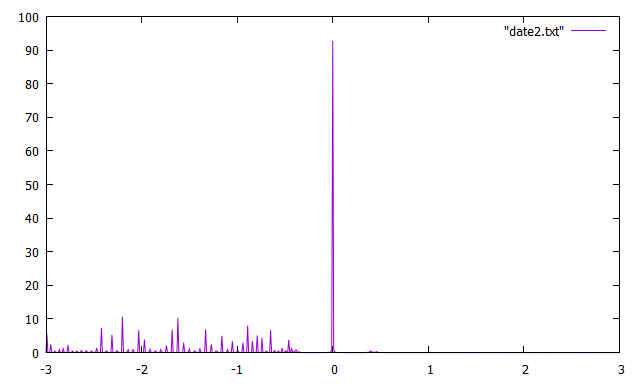
\includegraphics[scale=0.5]{LDOS3_bry.png}
                \caption{状態密度3(表面)}
                \label{LDOS3}
            \end{figure}

            \begin{figure}[H]
                \centering
                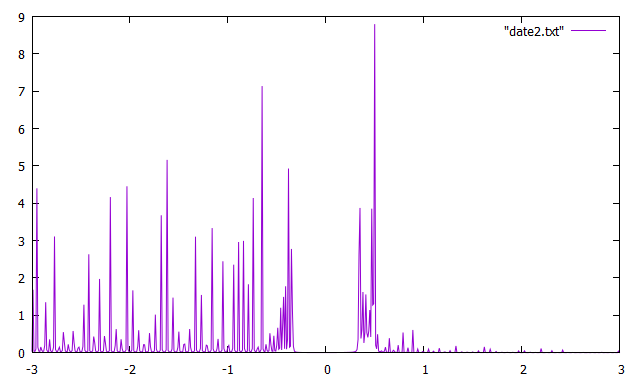
\includegraphics[scale=0.5]{LDOS3b_bry.png}
                \caption{状態密度3(バルク)}
                \label{LDOS3b}
            \end{figure}
        
         	図\eqref{LDOS3}から、表面ではE=0のときにピークが出ているのが分かる。それに対し図\eqref{LDOS3b}から、エネルギーが$-1$から$1$の範囲では状態がないことが分かる。これも2つ目のものと同様に、表面にエッジ状態があり、そこに電子が入ったためと考えられる。エッジ状態があるのは、図\eqref{Dispersion3}からも確認できる。また図\eqref{Dispersion3}を見てみると、(0,0)のところでエッジ状態か交差しているのがわかる。これは、表面の表と裏でクラマース対を作っていることが考えられる。

    \end{document}
    